%\documentclass[10pt,twoside]{article} %,draft
%
%\usepackage{latexsym,amsmath,amsfonts,amssymb,amsthm,graphics,epsfig,mathrsfs,zb2016,cite,color,enumerate,hhline}
%\usepackage{lscape}
%\usepackage[utf8x]{inputenc} %\usepackage[cp1251]{inputenc}
%\usepackage[warn]{mathtext}
%\usepackage[ukrainian]{babel}
%
%\usepackage[T2A]{fontenc}
%\usepackage{textcomp}
%\usepackage{epstopdf}
%\begin{document}

\section{Вступ}
Шановні автори, при підготовці публікацій у збірнику наукових праць "Вісник Національного технічного університету України "Київський політехнічний інститут". Серія Радіотехніка. Радіоапаратобудування" дотримуйтесь правил оформлення матеріалів, наведених у цьому прикладі правил оформлення (шукайте електронну версію на сайті збірника http://radap.kpi.ua/archive/Zrazok.doc).

Приклад оформлення посилань \cite{radap1354ref1,radap1354ref4}. 


\section{Вимоги до оформлення}

Оцінка ефективності моніторингових заходів в ІС ТКС останнім часом є предметом підвищеної уваги з боку вчених. З’явилася певна кількість статей, присвячених цьому питанню. В \cite{radap1354ref1} надані основи обробки й аналізу сигналів радіовипромінювань, визначені основи структурно-системного методу обробки сигналів радіовипромінювань. В \cite{radap1354ref2} описується використання алгоритмів нечіткого кластерного аналізу для забезпечення функціональної стійкості ієрархічного інформаційного процесу на етапі класифікації об’єктів радіомоніторингу. В \cite{radap1354ref3} досліджуються методи ідентифікації радіотехнічних вимірів при супроводі  близько розташованих об’єктів. В \cite{radap1354ref4} розглядаються методи розпізнавання і цифрової обробки відображень в ІС ТКС. В \cite{radap1354ref5} аналізуються методи моніторингу інформації в ІС ТКС. В \cite{radap1354ref6} викладені основні концепції, які визначають сучасний стан і тенденції розвитку комп’ютерних мереж. Але оцінці інформативності моніторингових ознак і сигнатур та мірі їх невизначеності при розпізнаванні джерел та об’єктів моніторингу достатньої уваги приділено не було. Світових досліджень щодо визначення інформаційної ефективності моніторингових ознак через ентропію автору невідомо. Автор сподівається, що разом із виданням цієї статті, такі відомості з'являться.

\section{Виклад основного матеріалу}

Для вирішення сформульованих завдань розглянемо процес розпізнавання системи $А$~--- джерела (об’єкта) моніторингу, яке випадково може належати деякому класу або перебувати у тому або іншому стані, тобто системи, що має деякий ступінь невизначеності~--- ентропію.

Стан (або належність до класу) системи оцінюється і визначається за параметрами відповідних МО~--- кількісних та якісних, які мають бути найбільш наближеними до еталонних~--- без втрат інформації, тобто мати мінімальний ступінь невизначеності~--- ентропію.

Відомо \cite{radap1354ref4}, що ентропія може бути оцінена як кількістю можливих станів $(х_1, х_2, \ldots, х_n)$ системи, так і величинами імовірностей цих станів $(р_1, р_2, \ldots, р_n)$, при цьому $\sum_{i=1}^{n}p_i=1$  де $n$~--- кількість станів:
\begin{equation}\label{radap1354eq1}
H(A)=-\sum \limits_{i=1}^n p_i \log p(p_i)
\end{equation}
яка: дорівнює нулю, коли один зі станів системи достовірний, а інші неможливі; досягає максимуму, якщо ці стани рівноімовірні $(р_1 = р_2 = \ldots = р_n)$; при збільшенні кількості станів зростає; ентропії систем сумують: $H(a) = -\sum_{i=1}^{n}H_i(A)$ .

Що стосується вибору основи логарифма, то взагалі він може мати значення при будь-якому $a \succ 1$, а його зміна еквівалентна обранню одиниці вимірювання ентропії. На сьогодні у галузях обчислювальної техніки, цифрового радіозв’язку, телекомунікаційних системах різного призначення для розрахунків та аналізу використовують логарифми з основою $а = 2$ і бінарну логіку та вимірюють ентропію у двійкових одиницях, що добре погоджується з двійковою системою числення (\textit{bit}~--- це ентропія одного розряду двійкового числа, якщо він з рівною (однаковою) імовірністю може бути $0$ або $1$). Однак у радіоелектронному моніторингу такий вибір $а = 2$ не завжди доцільний, що пояснюється великою кількістю можливих станів об’єктів або належністю джерел моніторингу до певного класу: $n \ge 2$. А якщо застосовуються вербальні (якісні) ознаки і логічні методи розпізнавання та підтримки прийняття рішення, необхідно використовувати методи багатозначної, а не бінарної логіки.

Рівняння \eqref{radap1354eq1} можна надати у такому вигляді:
\begin{equation}\label{radap1354eq2}
H(A)=-\sum \limits_{i=1}^n p_i \log (p_i) = \sum \limits_{i=1}^n p_i \log \frac{1}{p_i}
\end{equation}

Тоді величину $\frac{1}{p_i}$  можна розглядати як окрему ентропію, що характеризує інформативність ознаки за параметром $х_і$, а ентропію $Н$~--- як середнє значення окремих ентропій. При малих значеннях $р_і$ окрема ентропія велика, і з наближенням $р_і$ до одиниці вона прагне до нуля, а функція $[-p_i \log (p_i) ]$ відображає внесок ознаки $х_і$ до ентропії $Н$.

При цьому для розрахунків можна скористатися такими відомими співвідношеннями \cite{radap1354ref7}:
\begin{list}{-}{}
	\item ентропія рішення про належність або стан джерела об’єкту моніторингу (ДОМ) $А$ за параметром $x_k$  моніторингової ознаки визначається як
\begin{equation}\label{radap1354eq3}
H(A/x_k)=-\sum \limits_{k=1}^N p(A/x_k) \log p(A/x_k)  
\end{equation}
	де $p(A/x_k)$ ~--- умовна імовірність визначення належності або стану ДОМ $А$ за параметром $x_k$;
	
	\item умовна імовірність $p(A/x_k)$  знаходиться за формулою Байєса:
\begin{equation}\label{radap1354eq4}
p(A/x_k) = \frac{p(A)p(x_k/A)}{p(x_k)}
\end{equation}
	де $p(x_k) = \sum_{r=1}^{N} p(A)p(x_k/A)$ ~--- імовірність появи $k$-го параметра ознаки в усіх ДОМ;  $p(x_k/A)$~--- умовна імовірність появи  $k$-го параметра ознаки в системі $А$.
\end{list}

Інколи для зручності обчислювань \eqref{radap1354eq1} і \eqref{radap1354eq5} застосовують спеціальну функцію $\eta = - \log p(p)$ , тоді 
\begin{equation}\label{radap1354eq5}
H(A) = -\sum\limits_{i=1}^N \eta (p_i)
\end{equation}

Формули  \eqref{radap1354eq1},  \eqref{radap1354eq2} і \eqref{radap1354eq5} використовують для обчислення значення ентропії, однак для виконання математичних перетворень більш зручною є форма запису ентропії у вигляді математичного очікування $H(A)=M[-[\log P(A)]]$, де $Р(А)$~--- імовірність будь-якого (випадкового) стану системи.

Якщо система $А$ має стани $(х_1, х_2, \,\ldots\,, хn)$, то випадкова величина $\log P(A)$ буде мати значення:
\begin{equation}\label{radap1354eq6}
\log p_1, \log p_2, \log p_3, \,\ldots\, , \log p_n.
\end{equation}

Статистичне середнє значення (математичне очікування) випадкової величини $[-\log P(A)$] є ентропією системи $А$, і для її обчислення значення \eqref{radap1354eq6} усереднюються з ``вагами'', рівними відповідним імовірностям $p_1, p_2,\,\ldots\,, p_n$.

Для підтвердження викладеного розглянемо і проаналізуємо графічні залежності величини ентропії від імовірності стану системи (рис. 1). Крива 1 (симетрична відносно $р = 0,5$) відповідає випадку бінарного стану системи або належності до двох класів, тобто $n= 2$, $а = 2$ і ентропія досягає максимального значення $Н = 1$ при $р_1= р_2= 0,5$~--- ступінь невизначеності найбільший.

\begin{figure*}\centering%{l}{\linewidth}
	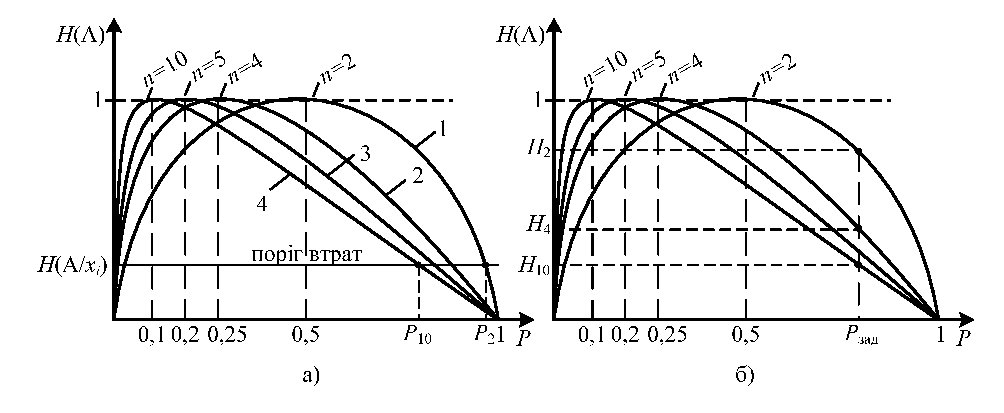
\includegraphics[width=0.75\linewidth]{fig1}
	
	\captionof{figure}{Залежності величини ентропії $Н(А)$ від імовірності $р$ стану системи}\label{fig1}
\end{figure*}

Якщо система має кількість станів $n \succ 2 $ , наприклад, $n = 4,5,10$, то відповідно для $n = 4$, $а = 4$ максимальна ентропія (ступінь невизначеності) $Н = 1$ досягається, коли $р_1 = р_2 = р_3 = р_4 = 0,25$ (крива 2); для $n = 5$, $а = 5$: $р_1 = р_2 = р_3 = р_4 = р_5 = 0,2$ (крива 3); для $n = 10$, $а = 10$: $р_1 = р_2 =\ldots= р_{10} = 0,1$ (крива 4). Як видно з наведених залежностей, максимум ентропії зі збільшенням $n \succ 2 $  зсувається ліворуч (порівняно з бінарним випадком 
$n= 2$, $а = 2$, $р_1= р_2= 0,5$).

Як було зазначено, при розпізнаванні для оцінювання інформаційної ефективності ознак і сигнатур зручніше використовувати поняття величини втрати інформації $\Delta I_x$ за параметром $х_і$ ознаки ДОМ~--- ступінь остаточної (кінцевої) невизначеності їх інформаційних параметрів або неповноту моніторингових ознак: 
\begin{equation}\label{radap1354eq7}
\Delta I_x = H_0(A)-H(A/x_i)
\end{equation}

Тоді інформаційна ефективність $Е_х$ моніторингової ознаки буде дорівнювати:
\begin{equation}\label{radap1354eq8}
E_x = \frac{H_0(A)-H(A/x_i)}{H_0(A)} = 1-\frac{H(A/x_i)}{H_0(A)}
\end{equation}
а інформаційна ефективність $Е_с$ сигнатури є середнім статистичним значенням сумарної ефективності сукупності моніторингових ознак:
\begin{equation}\label{radap1354eq9}
E_c = \frac{1}{n}\sum\limits_{j=1}^{n}E_{xj}
\end{equation}
де $n$~--- кількість МО у сигнатурі.
З виразу \eqref{eq8} випливає:
\begin{list}{-}{}
	\item якщо невизначеність за МО $х_і$ максимальна (інформаційні втрати значні), то $H(A/x_i) \to H_0(A)$  й інформаційна ефективність за цією ознакою зменшується, а імовірність правильного розпізнавання прагне до нуля;
	
	\item у випадку незначних інформаційних втрат ($\Delta I_x \to 0$; $H(A/x_i) \to 0$), тобто відсутності невизначеності за МО, інформаційна ефективність набуває максимального значення і прагне до одиниці.
\end{list}

Аналіз графічних залежностей (рис. \ref{fig1}) дає можливість зробити такі висновки:
\begin{itemize}
	\item інформаційна ефективність МО за відповідним параметром оцінюється втратами інформації~--- різницею між початковою ентропією $Н_0(А)$ та ентропією $Н_0(А/х_і)$ за параметром $х_і$, тобто ступенем невизначеності;
	
	\item при вирішенні завдань розпізнавання робоча область залежностей $Н = f(p)$ (рис. \ref{fig1}) міститься у правій напівплощині ($\eth \succ 0,5$);
	
	\item якщо встановити рівень порога для $Н(А/х_і)$, що визначає інформаційні втрати МО за параметром $х_і$, наприклад, $Н(А/х_і) = 0,1Н_0$, то можна оцінити потрібну величину імовірності $р$ для $n = 2, 4, 5, 10$ (рис. \ref{fig1}, а);
	
	\item у випадку, коли заданою є значення імовірності $р_{зад}$, за допомогою наведених кривих можна встановити інформаційні втрати відповідно для $n = 2, 4, 5, 10$ (рис. \ref{fig1}, б).
\end{itemize}

Тобто система $А$ зі станами $(х_1, х_2, \ldots , х_n)$ та імовірностями 
$(р_1, р_2, \ldots, р_n)$ за інформаційними параметрами МО і сигнатур описана та проаналізована досить повно як аналітично, так і графічно.

З урахуванням наведеного розглянемо процес і механізм оцінювання інформаційних втрат при формуванні сигнатур $СГ_1, СГ_2, \ldots, СГ_m$ на підставі отриманих моніторингових ознак $МО_{11}, МО_{12}, \ldots, МО_{1n}$ (рис. \ref{fig2}).



%\begin{wrapfig}\center%[htbp]
%	
%	

%\end{wrapfig}
\begin{Figure}%{l}{\linewidth}\centering
	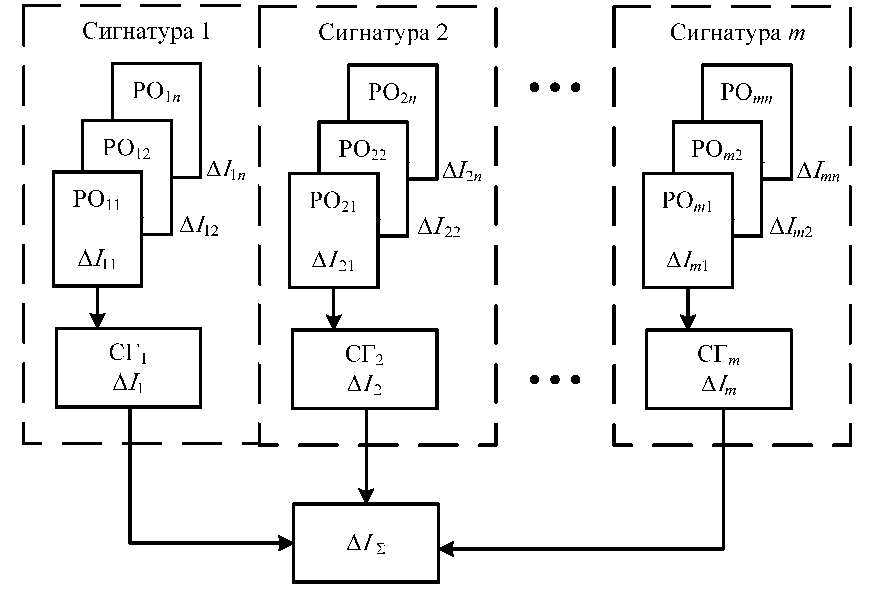
\includegraphics[width=\linewidth]{fig2}
		\captionof{figure}{Пояснення процесу оцінювання інформаційних втрат при формуванні сигнатур із сукупності моніторингових ознак}\label{fig2}
\end{Figure}

Згідно з основним змістом ССМ і СГСМ моніторинговими підрозділами добуваються моніторингові відомості і визначається множина МО (наприклад, параметричних: тривалість сигналів, їх частота, період або частота надходження імпульсів тощо). Отримані МО $(МО_{11}, МО_{12}, \ldots, МО_{1n})$ формують відповідні сигнатури $(СГ_1, СГ_2, \ldots, СГ_m)$, які використовуються у процесі розпізнавання і покладені в основу прийняття рішення про належність джерел до певного класу або оперативний (фазовий) стан об’єктів. 

Кожна моніторингова ознака $(МО_{11}, МО_{12},  $ $ \ldots, МО_{1n})$ має власні інформаційні втрати $(\Delta I_{11}, \Delta I_{12}, \ldots, \Delta I_{1m})$, а сформовані сигнатури $(СГ_1, СГ_2, \ldots, СГ_m)$~--- втрати $(\Delta I_{1}, \Delta I_{2}, \ldots, \Delta I_{m})$. Якщо ці втрати незначні, об’єкт моніторингу виявляється (його ентропія зменшується) із сумарною втратою інформації $\Delta I_{\sum}$, яка обумовлена насамперед похибками визначення, вимірювання й оцінювання параметрів моніторингових ознак ДРВ.

Описаний процес (рис. \ref{fig2}) розглянемо детальніше за допомогою графічних (рис. \ref{fig3}) та аналітичних залежностей при таких позначеннях: $k = 1, 2 \ldots j$~--- обсяг вибірки вимірювання або спостереження за параметром $х_і$ моніторингової ознаки з імовірностями $р_і$; $n = 1, 2, \ldots, i$~--- кількість моніторингових ознак у сигнатурі; $m= 1, 2, \ldots, s$~--- кількість сигнатур у процесі розпізнавання; перший індекс у $\Delta I_{mn}$  визначає номер сигнатури, другий~--- номер МО цієї сигнатури.


\begin{figure*}\centering
	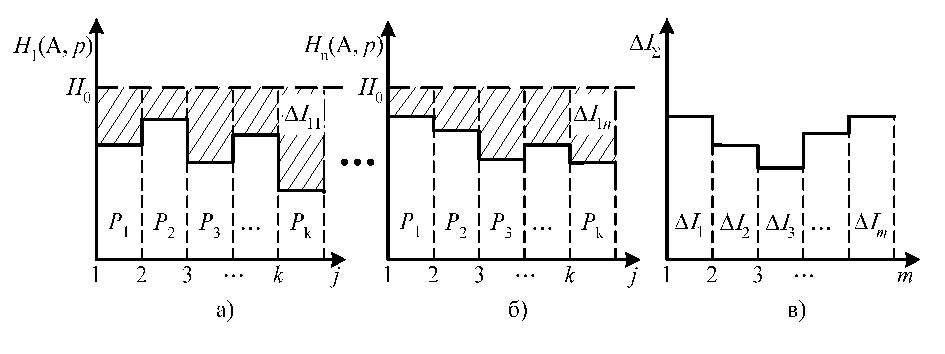
\includegraphics[width=0.8\linewidth]{fig3}
	
\captionof{figure}{Визначення інформаційних втрат $\Delta I_{1n}$ моніторингових ознак (а), (б)
		та сигнатур $\Delta I_{\sum}$  (в)}\label{fig3}
\end{figure*}


%	\begin{Figure}
%		\centering
%		\includegraphics[width=\linewidth]{foo}
%		\captionof{figure}{my caption of the figure}
%	\end{Figure}


Визначимо ентропії моніторингових ознак $МО_{1n}$ джерела випромінювання $А$ за параметром $х_і$ при обсягу вибірки $k$.

Величина ентропії моніторингової ознаки $МО_{11}$ за параметром $х_1$ дорівнює:
\begin{equation}\label{radap1354eq10}
H_1(A/x_1) = -\sum\limits_{j=1}^{k} p_j(A/x_{1j})\log p_j(A/x_{1j})
\end{equation}
ентропія $МО_{12}$ за параметром $х_2$: 
\begin{equation}\label{radap1354eq11}
H_2(A/x_2) = -\sum\limits_{j=1}^{k} p_j(A/x_{2j})\log p_j(A/x_{2j})
\end{equation}
ентропія $МО_{1n}$ за параметром $х_n$: 
\begin{equation}\label{radap1354eq12}
H_n(A/x_n) = -\sum\limits_{j=1}^{k} p_j(A/x_{nj})\log p_j(A/x_{nj})
\end{equation}

Відповідні інформаційні втрати цих ознак будуть мати такі значення:
\begin{equation}
\begin{aligned}\label{radap1354eq13}
\Delta I_{11} &= H_0(A)-H_1(A/x_1)\\ 
\Delta I_{12} &= H_0(A)-H_2(A/x_2)\\ 
\Delta I_{1n} &= H_0(A)-H_n(A/x_n)
\end{aligned}
\end{equation}

Статистичні середні значення (або математичне очікування при великому обсязі вибірки $k$) величини втрати інформації $ \Delta I_1, \Delta I_2 , \ldots, \Delta I_m $  сигнатур визначаються як
\begin{equation}\label{radap1354eq14}
\begin{matrix}
\Delta I_{1} = \frac{1}{n} \sum\limits_{i=1}^{n} \Delta I_{1i} \\
\Delta I_{2} = \frac{1}{n} \sum\limits_{i=1}^{n} \Delta I_{2i} \\
\Delta I_{m} = \frac{1}{n} \sum\limits_{i=1}^{n} \Delta I_{mi} 
\end{matrix}
\end{equation}

У результаті сумарні втрати інформації в процесі розпізнавання матимуть такі значення:
\begin{equation}\label{radap1354eq15}
\Delta I_{\sum} = \frac{1}{m}\sum\limits_{m=1}^{s} \Delta I_m  = \frac{1}{mn}\sum\limits_{m=1}^{s} \sum\limits_{n=1}^{s}\Delta I_{mn}   
\end{equation}

Слід зазначити, що наукове завдання визначення оптимального значення кількості моніторингових ознак $n$ для забезпечення максимального значення імовірності правильного розпізнавання $Р_{пр}$ під час моніторингу і розпізнавання ДРВп авторами вирішено, описано у \cite{radap1354ref1} і ця кількість дорівнює $n_{опт} = 4-5$, що добре узгоджується з результатами досліджень, викладених, наприклад, у \cite{radap1354ref4}.

Тоді на підставі розглянутого й отриманих аналітичних залежностей \eqref{radap1354eq12}, \eqref{radap1354eq13}, \eqref{radap1354eq14}, \eqref{radap1354eq15} при заданих значеннях $n = 4-5$, $Р_{пр} = const$~--- $max$ та $\Delta I = const$~--- $min$ можна просто та швидко розрахувати і побудувати залежності $\Delta I = f(m)$ , за якими визначити оптимальну або раціональну кількість сигнатур $m$ (рис.~4).


\begin{figure}[htbp]\center
	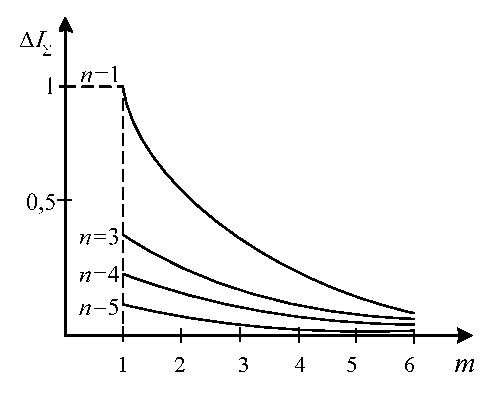
\includegraphics[width=0.6\textwidth]{fig4}
	
	\caption{Залежність сумарних інформаційних втрат  $\Delta I_{\sum}$
		від кількості сигнатур $m$ під час розпізнавання}\label{fig4}
\end{figure}


Аналіз наведених графічних залежностей (рис. \ref{fig4}) свідчить, що зі збільшенням кількості сигнатур $m$ інформаційні втрати зменшуються і при $m \succ 4$  практично не змінюються (втрати фіксуються на мінімальному рівні). Цей результат є цілком фізичним: якщо обрати $n_{опт} = 4-5$, а $m = 3\,–\,4$, то загальна кількість моніторингових ознак при розпізнаванні буде дорівнювати $n_{\sum} = n \times m = 12-20$, що призведе до зростання величини імовірності правильного розпізнавання $Р_{пр}$ при фіксованих похибках 1-го та 2-го роду.

\pdfbookmark[1]{Висновки}{conc}
\section*{Висновки}
Рукопис оформлений відповідно до цього шаблону слід надсилати у редакцію через офіційний сайт, після чого до Вас на електронну пошту прийде підтвердження отримання рукопису. Далі редактор виконає формальну перевірку рукопису на відповідність вимогам до оформлення статей та направить його на рецензування. Матеріали, що оформлені з відхиленнями від встановлених вимог можуть направляютися авторам на доопрацювання. У разі виникнення запитань звертайтесь до редакції за тел. \texttt{+380 44 204 93 29} або електронною поштою \texttt{radap@rtf.kpi.ua}.



\pdfbookmark[1]{Перелік посилань}{lit}
\section*{Перелік посилань}
\begin{enumerate}\footnotesize
		
	\item Аксенов Г. Н. Основы обработки и анализа сигналов РЕС. Основы структурно-системного метода обработки данных радиоизлучений / Г.Н.~Аксенов,  Ю.А.~Смирнов.~--  К.~: КВИРТУ ПВО, 1989.~-- 200 с.
	\item Шуренок В. А. Використання алгоритмів нечіткого кластерного аналізу для забезпечення функціональної стійкості ієрархічного інформаційного процесу на етапі класифікації об’єктів радіомоніторингу / В.А.~Шуренок // Збірник наукових праць Житомирського військового інституту імені С. П. Корольова.~-- 2013.~-- №7.~-- с. 61-69.
	\item Логачев С.В. Дослідження методів ідентифікації радіотехничніх вимірів при супроводі близько розташованих об’єктів / С.В.~Логачев, Г.В.~Худов, Р.В.~Дзюбчук  / Збірник наукових праць Житомирського військового інституту імені С.П. Корольова.~-- 2013.~-- №8.~-- С. 47--53.  
	\item Анисимов Б.В. Распознавание и цифровая обработка изображений  / Б.В.~Анисимов, В.Д.~Курчанов, В.К.~Злобин.~-- М.~: Высшая школа, 1993.~-- 295~с. 
	\item Гриняев С. В.  Борьба сетей /  С. В. Гриняев // Независимое военное обозрение.~-- 2002.~-- №2.~-- с. 11-13.
	\item Таненбаум Э. В. Компьютерные сети, 4-е изд. / Э. В. Таненбаум.~-- СПб.~: Питер, 2015.~-- 992 с.
	\item Вентцель Е.С. Теория вероятностей  /  Е.С.~Вентцель.~-- М.~: Наука, 1969.~-- 576 с.
\end{enumerate}

\pdfbookmark[1]{References}{translit}
\renewcommand{\refname}{References}

\begin{thebibliography}{9}\footnotesize

\bibitem{radap1354ref1} Aksenov G. N. and Smirnov Yu. A. (1989) \textit{Osnovy obrabotki i analiza signalov RES. Osnovy strukturno-sistemnogo metoda obrabotki dannykh radioizluchenii} [Basics of processing and analyzing signals RES. Fundamentals of structural and systematic data processing method of radio emissions], Kyiv, KVIRTU PVO, 200\,p.
\bibitem{radap1354ref2} Shurenok V. A.  (2013) Application of fuzzy cluster analysis algorithms for providing of hierarchical information process functional stability at the stage of radiomonitoring objects classification. \href{http://nbuv.gov.ua/UJRN/Psvz_2013_7_9}{\textit{Problemy stvorennia, vyprobuvannia, zastosuvannia ta ekspluatatsii skladnykh informatsiinykh system}}, No 7, pp. 61-68. (in Ukrainian) 
\bibitem{radap1354ref3} Logachov S. V., Hudov G. V. and Dzуubchuk R. V. (2013) The  research  of  the  methods  for  identification  of radiotechnical measurements accompanied by closely located space objects. \href{http://nbuv.gov.ua/UJRN/Psvz_2013_8_8}{\textit{Problemy stvorennia, vyprobuvannia, zastosuvannia ta ekspluatatsii skladnykh informatsiinykh system}}, No 8, pp. 47-53. (in Ukrainian)  
\bibitem{radap1354ref4} Anisimov B. V., Kurchanov V. D. and Zlobin V. K. (1993) \textit{Raspoznavanie i tsifrovaya obrabotka zobrazhenii} [The recognition and the digital Imaging],  Moskow, Vysshaya shkola, 295\,p. 
\bibitem{radap1354ref5} Grinyaev S. V. (2002) \textit{Bor'ba setei} [Fight of Networks]. Nezavisimoe voennoe obozrenie, No 2, pp. 11-13.
\bibitem{radap1354ref6} Tanenbaum E. V. (2015) \textit{Komp'yuternye seti} [Computer networks]. SPb., Piter, 992\,p.
\bibitem{radap1354ref7} Venttsel' E.S. (1969) \textit{Teoriya veroyatnostei} [The probability theory], Moskow, Nauka, 576\,p.

\end{thebibliography}

%\end{document}